% Partial sums of the Basel series against pi^2/6.
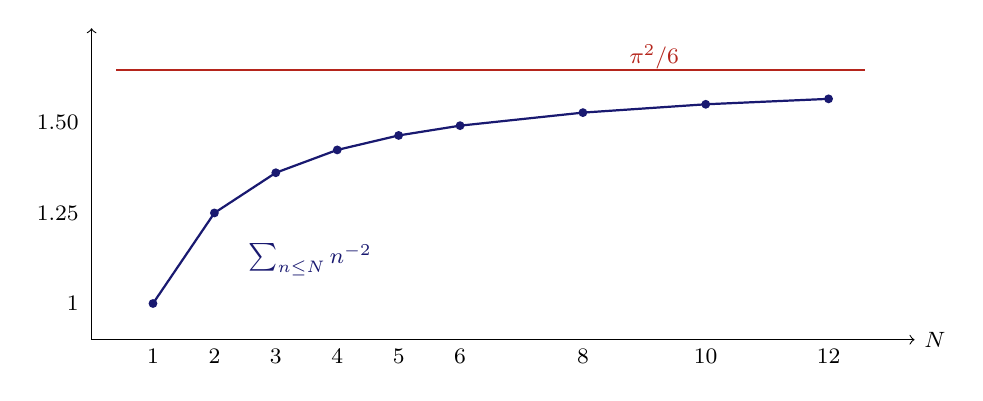
\begin{tikzpicture}[x=0.78cm,y=4.6cm,every node/.style={font=\footnotesize}]
  \draw[->,black] (0,0)--(13.4,0) node[right] {$N$};
  \draw[->,black] (0,0)--(0,0.86);
  \draw[BrickRed,thick] (0.4,0.745)--(12.6,0.745);
  \draw[MidnightBlue,thick]
    (1,0.100)--(2,0.350)--(3,0.461)--(4,0.524)--(5,0.564)--(6,0.591)
    --(8,0.627)--(10,0.650)--(12,0.665);
  \foreach \n/\y in {1/0.100,2/0.350,3/0.461,4/0.524,5/0.564,6/0.591,8/0.627,10/0.650,12/0.665} {
    \fill[MidnightBlue] (\n,\y) circle (1.6pt);
    \node[below] at (\n,0) {$\n$};
  }
  \node[anchor=east] at (-0.05,0.100) {$1$};
  \node[anchor=east] at (-0.05,0.350) {$1.25$};
  \node[anchor=east] at (-0.05,0.600) {$1.50$};
  \node[BrickRed,anchor=west] at (8.6,0.78) {$\pi^2/6$};
  \node[MidnightBlue,anchor=west] at (2.4,0.22) {$\sum_{n\le N}n^{-2}$};
\end{tikzpicture}
